%
% CHAPTER 3.- Codes and Information
%

\chapterimage{Morse_key.pdf}

\chapter{Coding}
\label{chap:Coding}

\begin{quote}
\begin{flushright}
\emph{Information is the resolution of uncertainty.}\\
Claude Shannon
\end{flushright}
\end{quote}
\bigskip

In this section, we review the conceptual foundations and main results of coding theory and the closely related field of information theory.

Coding is the process of representing a sequence of symbols from one alphabet by a sequence of symbols from another alphabet. Coding has many practical applications, such as error detection and correction, cryptography, and telecommunications. Our focus here is on data compression, that is, encoding a message using fewer symbols than in its original representation, while preserving all the information it contains. Compression algorithms reduce message size by identifying and eliminating statistical redundancies. For example, one may assign shorter descriptions to the most frequent symbols in the source and longer descriptions to the less frequent ones. A particular class of codes, known as prefix-free codes, will play a central role in this book. Prefix-free codes establish a natural connection between coding theory and probability theory, a connection that will be essential in the context of the theory of nescience.

Information theory proposes that the amount of information conveyed by the occurrence of an event is given by the negative logarithm of the probability of that event. In this sense, information can be interpreted as surprise: the less likely an event is, the more information we gain when it occurs. Although we will not adopt this interpretation of information in the theory of nescience, we will rely extensively on another fundamental concept from information theory: entropy. Entropy quantifies the uncertainty in the value of a random variable or the outcome of a random process. It is particularly relevant because it establishes a fundamental bound on compression: no code can achieve an average word length smaller than the entropy of the source alphabet.

There exist many interesting concepts derived from entropy, like joint entropy, conditional entropy, or mutual information. However, these concepts are more relevant in the context of communication because they allow us to solve the problem of how to transmit information in a reliable manner over a noisy channel. Here, they are introduced for completeness purposes, and to compare them with our own definitions of joint nescience and conditional nescience.

Several additional concepts are derived from entropy, including joint entropy, conditional entropy, and mutual information. These quantities play a central role in communication theory, as they are instrumental in addressing the problem of transmitting information reliably over noisy channels. In this book, however, they are introduced primarily for completeness and as a basis for comparison with our own definitions of joint nescience and conditional nescience.

%
% Section: Codes and their properties
%

\section{Coding}
\label{Codes}

Intuitively, coding refers to the process of losslessly describing a sequence of symbols (a message) from some alphabet by another sequence of symbols from a (possibly different) alphabet. There is no universal agreement on what exactly constitutes a code, as different authors propose different definitions in the literature. Fortunately, the definition of a prefix-free code (the kind of code used in the theory of nescience) is standard and widely accepted.

Let $\mathcal{S}=\left\{ s_{1},s_{2},\ldots,s_{q}\right\}$ be a finite set called the \emph{source alphabet}\index{Source alphabet}, and let $\mathcal{X}=\left\{ x_{1}, x_{2}, \ldots, x_{r} \right\}$ be a finite set called the \emph{code alphabet}\index{Code alphabet}.

\begin{definition}[Code]
A \emph{code}\index{Code} for $\mathcal{S}$ is a total function $C:\mathcal{S}\rightarrow\mathcal{X}^{+}$. If $(s,x) \in C$ we say that $s$ is a \emph{source symbol}\index{Source symbol} and $x$ is the corresponding \emph{code word}\index{Code word}. If $C$ is injective, we say that the code is \emph{nonsingular}\index{Non-singular code}.
\end{definition}

Nonsingularity ensures that each symbol in the source alphabet is represented by a distinct code word, allowing us to unambiguously describe the individual symbols of the source alphabet. In what follows, unless otherwise stated, the term \emph{code} will always mean a nonsingular code. Moreover, without loss of generality, we restrict our discussion to \emph{binary codes}, that is, $\mathcal{X} = \mathcal{B} = \{0, 1\}$.

The property of nonsingularity can also be extended from individual symbols to strings of symbols. For that, we introduce the notion of extensions of a code.

\begin{definition}
The \emph{extension of order $n$} of a code $C$\index{Code extension} is a function $C^{n}:\mathcal{S}^{n}\rightarrow\mathcal{B}^{+}$ defined by
\[
C^{n}(s_{i_1} \ldots s_{i_n}) = C(s_{i_1}) \ldots C(s_{i_n}),
\]
where the right-hand side is the concatenation of the code words corresponding to the symbols $s_{i_1} \ldots s_{i_n} \in \mathcal{S}^{n}$. An extension of order $n$ is \emph{nonsingular} if $C^{n}$ is injective.
\end{definition}

If it is clear from the context, we will also use the word \emph{code} to refer to a nonsingular extension of order $n$ of a code, and the elements of \(\mathcal{S}^{n}\) will be called \emph{source words}.

\begin{example}
\label{ex:nonsingularity}
The code defined by $C(a)=0$, $C(b)=00$, $C(c)=01$, and $C(d)=11$ is nonsingular, but its extension of order $2$ is singular, since $C^2(ab)=C^2(ba)=000$.
\end{example}

As Example \ref{ex:nonsingularity} illustrates, not all nonsingular codes have nonsingular extensions. In such cases, it may be impossible to recover the original message from its encoded version. To address this, we introduce the stronger property of unique decodability.

\begin{definition}
A code $C$ is \emph{uniquely decodable}\index{Uniquely decodable code} if its extension $C^{n}$ is nonsingular for all $n$.
\end{definition}

The following proposition provides a useful characterization of unique decodability.

\begin{proposition}
A code $C$ is uniquely decodable if and only if the function $C^{+}:\mathcal{S}^{+}\rightarrow\mathcal{B}^{+}$ is injective.
\end{proposition}
\begin{proof}
If $C^{+}$ is injective, then every restriction $C^{n}$ is injective, and the code is uniquely decodable.  

Conversely, assume that $C^{n}$ is nonsingular for all $n$. Suppose, for contradiction, that $C^{+}$ is not injective. Then there exist two source words $s_{1} \in \mathcal{S}^{n}$ and $s_{2} \in \mathcal{S}^{m}$ with $n \neq m$ such that $C^{+}(s_{1}) = C^{+}(s_{2})$. Construct $s_{3} = s_{1}s_{2}$ and $s_{4} = s_{2}s_{1}$. Both have the same length, but
\[
C^{+}(s_{3}) = C^{+}(s_{1})C^{+}(s_{2}) = C^{+}(s_{2})C^{+}(s_{1}) = C^{+}(s_{4}),
\]
contradicting the injectivity of $C^{n+m}$. Therefore $C^{+}$ must be injective.
\end{proof}

\begin{example}
\label{ex:uniquely-decodable}
The code $C(a)=0$, $C(b)=01$, $C(c)=011$, and $C(d)=0111$ is uniquely decodable. For example, the code word $0010011$ corresponds uniquely to the source word $abac$. Unique decodability is achieved because the leading $0$ acts as a delimiter, separating code words.
\end{example}

The Sardinas-Patterson theorem provides a necessary and sufficient condition for unique decodability. The theorem is based on an algorithmic construction that examines successive sets of possible ambiguities.

Let $C_0$ denote the set of code words of a code $C$. Define
\[
C_n = C^{-1} C_{n-1} \cup C_{n-1}^{-1} C,
\]
for all $n \in \mathbb{N}$, where $C^{-1}D = \{ y \mid \exists x \in C, \, xy \in D \}$ is the left quotient of $C$ and $D$. Finally, let
\[
C_\infty = \bigcup_{n=1}^{\infty} C_n.
\]

\begin{proposition}[Sardinas-Patterson]\index{Sardinas-Patterson}
A code $C$ is uniquely decodable if and only if $C_0 \cap C_\infty = \varnothing$.
\end{proposition}
\begin{proof}
If $C_0 \cap C_\infty \neq \varnothing$, then there exists a nonempty overlap between some code word and a concatenation of code words, implying that at least two distinct source words map to the same encoded string, so $C$ is not uniquely decodable.  

Conversely, if $C_0 \cap C_\infty = \varnothing$, then the iterative construction guarantees that no ambiguity arises in the decoding process, regardless of message length. Therefore the code is uniquely decodable.  
\end{proof}

\begin{example}
For the code of Example \ref{ex:nonsingularity}:
\begin{align*}
 & C_0 = \{0, 00, 01, 11\} \\
 & C_1 = \{0, 1\}
\end{align*}
Since $C_0 \cap C_1 \neq \varnothing$, the code is not uniquely decodable.

For the code of Example \ref{ex:uniquely-decodable}:
\begin{align*}
 & C_0 = \{0, 01, 011, 0111\} \\
 & C_1 = \{1, 11, 111\} \\
 & C_2 = \varnothing
\end{align*}
Here $C_0 \cap C_\infty = C_0 \cap \bigcup^\infty_{n=1} C_n = C_0 \cap C_1 = \varnothing$, so the code is uniquely decodable.
\end{example}

Next definition introduces the concept of prefix-free codes. Prefix-free codes will play a critical role in the computation of the amount of algorithmic information of an arbitrary string (described in Chapter \ref{chap:Algorithmic_Information}), and in our own theory of nescience. Prefix-free codes also allow us to link coding theory and probability theory through the Kraft inequality (Theorem \ref{th:Kraft-Inequality}). Note that we prefer the name \emph{prefix-free code} over the more standard \emph{prefix code}, since the former more accurately describes the concept.

\begin{definition}[Prefix-free Code]\index{Prefix-free code}
\label{def:Prefix-free-Code}
A code $C$ is \emph{prefix-free} if for all $i, j$ whth $1 \leq i, j \leq q$ and $i \neq j$, $C(s_i)$ is not a prefix of $C(s_j)$.
\end{definition}

Note that the fact that a string is a prefix of itself does not violate the prefix-free property, because the condition specifically excludes considering a string as a prefix of itself ($i \neq j$) when determining whether a set of code words is prefix-free.

\begin{example}
\label{ex:prefix-free}
The code $C(a)=0$, $C(b)=10$, $C(c)=110$, and $C(d)=1110$ is prefix-free. Here, the symbol $0$ plays the role of a delimiter (as in Example \ref{ex:uniquely-decodable}), but placing it at the end of each code word ensures that no code word can be a prefix of another.
\end{example}

Prefix-free codes are uniquely decodable, as the next proposition shows.

\begin{proposition}
Let $C$ be a prefix-free code. Then $C$ is uniquely decodable.
\end{proposition}
\begin{proof}
Assume, for contradiction, that $C$ is not uniquely decodable. Then there exist two distinct sequences $r \neq s$ of source symbols such that $C(r)=C(s)$. Among all such pairs, choose one with the minimal common encoded length. Let $r = a r'$ and $s = b s'$ with $a \neq b$ (if $a=b$, cancel the common first symbols to get a shorter counterexample, contradicting minimality). Then $C(a)$ is a prefix of $C(b)C(s')$ and $C(b)$ is a prefix of $C(a)C(r')$. In particular, one of $C(a)$ or $C(b)$ must be a prefix of the other, contradicting the prefix-free property. Hence $C$ must be uniquely decodable.
\end{proof}

From an engineering point of view, it is highly convenient to have codes whose source symbols can be decoded as soon as the corresponding code words are received. In other words, it should not be necessary to wait for the next code word in order to decode the current symbol. For this reason, some authors refer to these codes as \emph{instantaneous codes}.

\begin{definition}
A code $C$ is \emph{instantaneous} if, for any order $n$ and for any sequence of code words $C(s_{i_1}), C(s_{i_2}), \ldots, C(s_{i_n})$, each sequence of code words $\mathbf{t} = C(s_{i_1})C(s_{i_2})\ldots C(s_{i_m})\ldots$ can be uniquely decoded as $\mathbf{s} = s_{i_1}s_{i_2}\ldots s_{i_m}\ldots$ without ambiguity, regardless of the continuation of $\mathbf{t}$.
\end{definition}

\begin{example}
The code described in Example \ref{ex:uniquely-decodable} is not instantaneous. For instance, after receiving the sequence $011$, the decoded symbol could be $c$ if the next bit is $0$ or $d$ if it is $1$; thus, one must look ahead to decide.
\end{example}

Prefix-free codes and instantaneous codes are essentially two terms for the same concept. A prefix-free code is one in which no code word is a prefix of any other code word. This ensures a clear boundary between consecutive code words, allowing immediate decoding upon receipt.

\begin{proposition}
A code $C$ is instantaneous if and only if it is prefix-free.
\end{proposition}
\begin{proof}
Suppose $C$ is instantaneous but not prefix-free. Then there exist at least a pair of code words, say $C(s_i)$ and $C(s_j)$, such that $C(s_i)$ is a prefix of $C(s_j)$. Consider a sequence where $C(s_j)$ is transmitted. Since $C(s_i)$ is a prefix of $C(s_j)$, the decoder would decode $C(s_i)$ from the initial part of $C(s_j)$, leading to ambiguity, as the rest of $C(s_j)$ could be seen as another code or part of the next code. This contradicts the assumption that $C$ is instantaneous.

Suppose $C$ is prefix-free. Reading a concatenation of code words from left to right, the first position at which a code word ends is unambiguous, because no longer code word can have the current code word as a prefix. Thus each code word can be decoded immediately upon completion, with no lookahead. Hence $C$ is instantaneous.
\end{proof}

The last type of codes we review are fixed-length codes. We will use fixed-length codes to compute the length of a text when there are no regularities we can exploit to compress it.

\begin{definition}
\label{def:Fixed-Length-Codes}\index{Fixed-length code}
If all the code words of a code have the same length, we say that the code is a \emph{fixed-length code}.
\end{definition}

Fixed-length codes are prefix-free (and therefore instantaneous).

\begin{proposition}
Let $C$ be a fixed-length code, then $C$ is prefix-free.
\end{proposition}
\begin{proof}
Let $C$ be a fixed length code, and $C(s_i)$ and $C(s_j)$ the code words of two arbitrary source words $s_i$ and $s_j$. Assume that $C(s_i) <_p C(s_j)$, given the fact that $l(C(s_i)) = l(C(s_j))$ we have that $C(s_i) = C(s_j)$ and so, the code $C$ is prefix-free.
\end{proof}

Of course, the converse does not hold: not all prefix-free codes are fixed-length. The code in Example \ref{ex:prefix-free} is prefix-free but not fixed-length.

Figure \ref{fig:Classification-Codes} provides a graphical representation of the relationships among the different types of codes introduced in this section.

\begin{figure}[t]
\centering
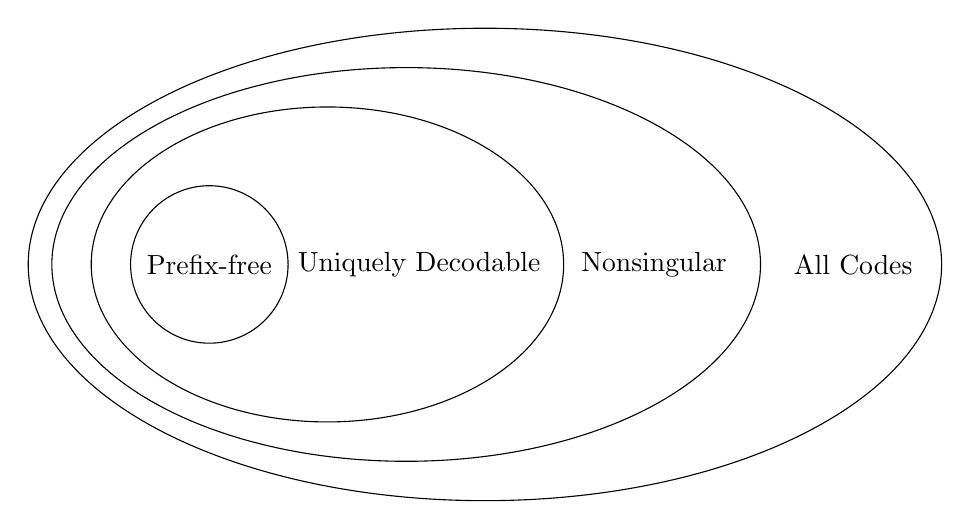
\begin{tikzpicture}
  % Draw the outer circle for "All Codes"
  \draw (3,0) ellipse (5.8cm and 3cm) node[right,xshift=3.8cm] {All Codes};

  % Draw the middle circle for "Nonsingular Codes"
  \draw (2,0) ellipse (4.5cm and 2.5cm) node[right,xshift=2.1cm] {Nonsingular};

  % Draw the inner circle for "Uniquely Decodable Codes"
  \draw (1,0) ellipse (3cm and 2cm) node[right, xshift=-0.5cm] {Uniquely Decodable};

  % Draw the most inner circle for "Prefix-free Codes"
  \draw (-0.5,0) ellipse (1cm and 1cm) node {Prefix-free};

\end{tikzpicture}
\caption{\label{fig:Classification-Codes}Classification of Codes}
\end{figure}

% \begin{figure}[t]
% \centering
% \begin{tikzpicture}
%   % Draw the outer circle for "All Codes"
%   \draw (3,0) ellipse (6cm and 3cm) node[right,xshift=3.8cm] {All Codes};

%   % Draw the middle circle for "Nonsingular Codes"
%   \draw (2,0) ellipse (4.5cm and 2.5cm) node[right,xshift=2.1cm] {Nonsingular};

%   % Draw the inner circle for "Uniquely Decodable Codes"
%   \draw (1,0) ellipse (3cm and 2cm) node[right, xshift=-0.5cm] {Uniquely Decodable};

%   % Draw the most inner circle for "Prefix-free Codes"
%   \draw (-0.5,0) ellipse (1cm and 1cm) node {Prefix-free};

% \end{tikzpicture}
% \caption{\label{fig:Classification-Codes}Classification of Codes}
% \end{figure}

%
% Section: Kraft Inequality
%

\section{Kraft Inequality}

The Kraft inequality provides a condition for the existence of a prefix-free code given a set of code word lengths. Kraft's inequality states that for a given set of code word lengths in a binary code, the sum of the reciprocals of powers of two corresponding to the code word lengths must be less than or equal to one. This condition is both necessary and sufficient: any prefix-free code must satisfy this inequality, and given a set of lengths that meets this condition, it is always possible to construct a corresponding prefix-free code. The elegance and utility of Kraft's inequality lie in its ability to link the lengths of code words with probabilistic structure.

\begin{figure}[t]
\centering
\begin{tikzpicture}[grow=right,->,>=stealth',level/.style={sibling distance = 3.2cm/#1,
  level distance = 2.5cm}] 
\node [circle,draw] (n1){}
    child{node [circle,draw] (n2) {$0$}
    }
    child{node [circle,draw] (n3) {$1$}
        child{node [circle,draw] (n4) {$10$}}
        child{node [circle,draw] (n5) {$11$}
            child{node [circle,draw] (n6) {$110$}}
            child{node [circle,draw] (n7) {$111$}
                child{node [circle,draw] (n8) {$1110$}}
            }
        }
    };
    
% Now, we add the edge labels
\path (n1) -- (n2) node [midway, above]  {$0$};
\path (n1) -- (n3) node [midway, above] {$1$};
\path (n3) -- (n4) node [midway, above]  {$0$};
\path (n3) -- (n5) node [midway, above] {$1$};
\path (n5) -- (n6) node [midway, above] {$0$};
\path (n5) -- (n7) node [midway, above] {$1$};
\path (n7) -- (n8) node [midway, above] {$0$};
\end{tikzpicture}
\caption{\label{fig:Prefix-Free-Tree}Prefix-free Tree}
\end{figure}

% \begin{figure}[t]
% \centering
% \begin{tikzpicture}[grow=right,->,>=stealth',level/.style={sibling distance = 4cm/#1,
%   level distance = 3cm}] 
% \node [circle,draw] (n1){}
%     child{node [circle,draw] (n2) {$0$}
%     }
%     child{node [circle,draw] (n3) {$1$}
%         child{node [circle,draw] (n4) {$10$}}
%         child{node [circle,draw] (n5) {$11$}
%             child{node [circle,draw] (n6) {$110$}}
%             child{node [circle,draw] (n7) {$111$}
%                 child{node [circle,draw] (n8) {$1110$}}
%             }
%         }
%     };
    
% % Now, we add the edge labels
% \path (n1) -- (n2) node [midway, above]  {$0$};
% \path (n1) -- (n3) node [midway, above] {$1$};
% \path (n3) -- (n4) node [midway, above]  {$0$};
% \path (n3) -- (n5) node [midway, above] {$1$};
% \path (n5) -- (n6) node [midway, above] {$0$};
% \path (n5) -- (n7) node [midway, above] {$1$};
% \path (n7) -- (n8) node [midway, above] {$0$};
% \end{tikzpicture}
% \caption{\label{fig:Prefix-Free-Tree}Prefix-free Tree}
% \end{figure}

\begin{theorem}[Kraft Inequality]
\label{th:Kraft-Inequality}
\index{Kraft's inequality}
Let $\mathcal{L}=\left\{ l_{1},l_{2},\ldots,l_{q}\right\}$ be a set of lengths, where $l_{i}\in\mathbb{N}$, then there exists a binary prefix-free code $C$ whose code words have the lengths of $\mathcal{L}$ if, and only if,
\[
\sum_{l_{i}\in\mathcal{L}}2^{-l_{i}}\leq1
\]
\end{theorem}
\begin{proof}
Consider a binary tree whose branches are labeled with the symbols of the code alphabet, in such a way that the path from the root to the leaves traces out the symbols of a code word. The prefix-free condition implies that nodes representing complete code words cannot have descendants. An example of such a tree, for the code described in Example \ref{ex:prefix-free}, is shown in Figure \ref{fig:Prefix-Free-Tree}.

Let $l_{max}=\max \left\{ l_{1},l_{2},\ldots,l_{q}\right\}$, that is, the length of the longest code word from the set of lengths. There will be at most $2^{l_{max}}$ leaf nodes in the tree, but at level $l_{i}$ we have to prune $2^{l_{max} - l_{i}}$ leaves, since the code is prefix-free. Summing over all the code words' lengths, we have that the total number of pruned leaves must be less than or equal to the maximum number of leaves, that is
\[
\sum_{l_{i}\in\mathcal{L}}2^{l_{max}-l_{i}} \leq 2^{l_{max}}
\]
or, equivalently,
\[
\sum_{l_{i}\in\mathcal{L}}2^{-l_{i}} \leq 1
\]
which is exactly the inequality we are trying to prove.

Conversely, given any set of code words' lengths $\mathcal{L}=\left\{ l_{1},l_{2},\ldots,l_{q}\right\}$ that satisfy the Kraft inequality, we can always construct a binary tree, like the one in the Figure \ref{fig:Prefix-Free-Tree}. Label the first node (lexicographically) of depth $l_{1}$ as code word 1, and remove its descendants from the tree. Then label the first remaining node of depth $l_{2}$ as code word 2, and so on. Proceeding this way, we construct a prefix code with the specified lengths.
\end{proof}

Given a code $C$ whose code word lengths $\mathcal{L}$ satisfy the Kraft inequality does not necessarily mean that the code is prefix-free, since what the inequality states is that there exists a prefix-free code with those word lengths, not that all codes with those word lengths are prefix-free.

\begin{example}
\label{ex:not-prefix-fix}
The code $C(a)=0$, $C(b)=111$, $C(c)=110$ and $C(d)=100$ satisfies the Kraft inequality, but it is not prefix-free.
\end{example}

McMillan's inequality extends Kraft's bound to all uniquely decodable codes: any such code with lengths \(l_i\) satisfies \(\sum_i 2^{-l_i}\le 1\). Combined with Kraft's theorem, this means a set of lengths meets this inequality if and only if it can be realized by a prefix-free---and thus uniquely decodable---code.

\begin{theorem}[McMillan's Inequality]
\index{McMillan's Inequality}
\label{th:McMillan-Inequality}
Let $\mathcal{L}=\left\{ l_{1},l_{2},\ldots,l_{q}\right\}$ be a set of lengths, where $l_{i}\in\mathbb{N}$, then there exists a uniquely decodable code $C$ whose code words have the lengths of $\mathcal{L}$ if, and only if,
\[
\sum_{l_{i}\in\mathcal{L}}2^{-l_{i}} \leq 1
\]
\end{theorem}
\begin{proof}
Let $S=\sum_{i=1}^q 2^{-l_i}$. For each $n\in\mathbb{N}$, let $C^n$ be the set of all concatenations of $n$ code words. Because the code is uniquely decodable, distinct concatenations in $C^n$ produce distinct binary strings. Consider an infinite fair-coin binary sequence $X=(X_1,X_2,\ldots)$, and for any finite binary string $u$ write $[u]=\{X:\, X \text{ begins with } u\}$. Then $\mathbb{P}([u])=2^{-|u|}$, and the cylinder sets $\{[w]: w\in C^n\}$ are pairwise disjoint. Therefore,
\[
\sum_{w\in C^n} 2^{-|w|} \;=\; \sum_{w\in C^n} \mathbb{P}([w]) \;\le\; 1.
\]
But the left-hand side factors as
\[
\sum_{w\in C^n} 2^{-|w|} \;=\; \Big(\sum_{i=1}^q 2^{-l_i}\Big)^n \;=\; S^n.
\]
Hence $S^n\le 1$ for all $n$, which implies $S\le 1$.
\end{proof}

In the theory of nescience, we focus on prefix-free codes without loss of generality: every uniquely decodable code satisfies Kraft's inequality, so there exists a prefix-free code with the same code-word lengths.

\begin{corollary}
There is an instantaneous (prefix-free) code with word lengths $l_1, \ldots, l_q$ if and only if there is a uniquely decodable code with these word lengths.
\end{corollary}
\begin{proof}
Every prefix-free code is uniquely decodable.

If a uniquely decodable code exists with lengths $l_1,\ldots,l_q$, then by McMillan's inequality $\sum_i 2^{-l_i}\le 1$. By Theorem \ref{th:Kraft-Inequality} (sufficiency), there exists a prefix-free code with the same lengths.
\end{proof}

In the context of nescience, our interest lies not in particular code assignments but in the multiset of code word lengths. This emphasis lets us abstract away from code construction details and focus on the mathematical properties of lengths, which are central to the measures we will use.

%
% Section: Optimal Codes
%

\section{Optimal Codes}
\label{sec:Optimal-Codes}

In coding theory, a compact code is an optimal encoding strategy that minimizes the expected length of code words, a concept central to evaluating a code's efficiency. The expected length of a code is determined by the weighted average of the lengths of its code words, with weights corresponding to the probability distribution of the source symbols. By designing code words so that more frequent symbols are assigned shorter lengths and less frequent ones longer lengths, compact codes effectively reduce the average size needed to encode information. This principle is pivotal in data compression, as it allows for a significant reduction in the space required for storage or the bandwidth needed for transmission.

Let $\mathcal{S}=\{ s_{1},\ldots,s_{q}\}$ be a finite source alphabet, and let $P$ be a probability distribution on $\mathcal{S}$.

\begin{definition}
The \emph{expected length}\index{Expected length of a code} of a code $C$, denoted by $L_{C}$, is
\[
L_{C} \;=\; \sum_{i=1}^{q} P(s_{i})\,l_{i},
\]
where $\mathcal{L} = \{ l_{1},\ldots,l_{q}\}$ are the code-word lengths of $C$. We may simply write $L$ when $C$ is clear from context.
\end{definition}

Our goal is to identify a code $C$ that minimizes $L$ under $P$. Such a code is optimal for $\mathcal{S}$ and $P$.

Compact codes achieve the lowest possible weighted average codeword length.

\begin{definition}
A code $C$ is \emph{compact}\index{Compact code} (optimal) if, for the given source alphabet $\mathcal{S}$ and distribution $P$, its expected length $L_{C}$ is minimal among all codes over the same code alphabet.
\end{definition}

The existence of compact codes for all possible source alphabets is a foundational aspect of coding theory, suggesting that for every finite source alphabet, an optimally efficient encoding scheme can be devised.

\begin{proposition}
For every finite source alphabet $\mathcal{S}$ and distribution $P$ there exists at least one code $C$ that is compact.
\end{proposition}
\begin{proof}
Huffman's algorithm (see Section \ref{sec:Huffman-Algorithm}) constructs a prefix-free code that minimizes the expected length for the given $P$. Hence an optimal code exists.
\end{proof}

It is convenient to distinguish between \emph{coding efficiency} and \emph{redundancy} relative to the source entropy. Let $H_r(P)=-\sum_i P(s_i)\log_r P(s_i)$ be the $r$-ary entropy (logarithms base $r$, where $r$ is the code alphabet size).

\begin{definition}
The \emph{coding efficiency} is
\[
\eta \;=\; \frac{H_r(P)}{L}\in(0,1],
\]
and the (normalized) \emph{redundancy} is
\[
\rho \;=\; 1-\eta \;=\; \frac{L-H_r(P)}{L}\in[0,1).
\]
\end{definition}

Our aim is to \emph{maximize} efficiency (equivalently, \emph{minimize} redundancy). Note that $L\ge H_r(P)$ (Theorem \ref{th:optimal_codes} below), so $\eta\le 1$.

Next theorem states that the entropy of the probability distibution $P$ poses a limit to the average length of prefix-free codes.

\begin{theorem}
\label{th:optimal_codes}
For any prefix-free $r$-ary code with lengths $\{l_i\}$ and source distribution $P$,
\[
H_{r}(P) \;\le\; L \;=\; \sum_{i=1}^{q} P(s_i)l_i,
\]
with equality if and only if $r^{-l_{i}} = P(s_i)$ for all $i$.
\end{theorem}
\begin{proof}
Let $\alpha=\sum_{i} r^{-l_i}\le 1$ by Kraft's inequality. Define a probability distribution $\tilde{Q}$ by
\[
\tilde{Q}(s_i)\;=\;\frac{r^{-l_i}}{\alpha}.
\]
Then
\begin{equation*}
\begin{split}
L - H_r(P)
& = \sum_i P(s_i)\Big(l_i + \log_r P(s_i)\Big) \\
& = \sum_i P(s_i)\log_r\!\Big(\frac{r^{l_i}P(s_i)}{1}\Big)
= \sum_i P(s_i)\log_r\!\Big(\frac{P(s_i)}{r^{-l_i}}\Big).
\end{split}
\end{equation*}
Write $r^{-l_i}=\alpha\,\tilde{Q}(s_i)$ to get
\begin{equation*}
\begin{split}
L - H_r(P)
& = \sum_i P(s_i)\log_r\!\Big(\frac{P(s_i)}{\tilde{Q}(s_i)}\Big)
\;+\; \log_r\!\Big(\frac{1}{\alpha}\Big) \\
& = D_r\!\big(P\;\|\;\tilde{Q}\big) \;+\; \log_r(1/\alpha)\;\ge\;0,
\end{split}
\end{equation*}
since the $r$-ary Kullback–Leibler divergence $D_r$ is nonnegative and $\alpha\le 1$. Equality holds iff both terms vanish, i.e., $\alpha=1$ and $P=\tilde{Q}$, which is equivalent to $r^{-l_i}=P(s_i)$ for all $i$.
\end{proof}

In data compression we are particularly interested in $r$-adic distributions.

\begin{definition}
A distribution $P$ is called \emph{$r$-adic} if each $P(s_i)$ is an exact $r$-adic probability, i.e., $P(s_i)=r^{-n_i}$ for some integers $n_i \ge 0$.
\end{definition}

Equality in Theorem \ref{th:optimal_codes} occurs precisely for sources whose symbol probabilities are exact powers of $r^{-1}$.

\begin{corollary}
Equality $L=H_r(P)$ in Theorem \ref{th:optimal_codes} holds if and only if $P$ is $r$-adic (equivalently, there exists a prefix-free code with $l_i=-\log_r P(s_i)$).
\end{corollary}
\begin{proof}
Theorem \ref{th:optimal_codes} shows equality holds exactly when $r^{-l_i}=P(s_i)$ for all $i$, i.e., when each $P(s_i)$ is an $r$-adic probability.
\end{proof}

In analysis it is natural to consider the \emph{ideal} real-valued lengths $\ell_i^\ast=-\log_r P(s_i)$, which need not be integers. Choosing integer lengths $l_i=\lceil \ell_i^\ast\rceil$ yields a feasible prefix-free code (by Kraft) with near-optimal average length.

\begin{proposition}[Shannon–Fano bound]
For $l_i=\lceil -\log_r P(s_i)\rceil$,
\[
H_r(P) \;\le\; L \;<\; H_r(P)+1.
\]
\end{proposition}
\begin{proof}
By definition $l_i< -\log_r P(s_i)+1$, hence
\[
L=\sum_i P(s_i)l_i \;<\; \sum_i P(s_i)\big(-\log_r P(s_i)+1\big) \;=\; H_r(P)+1.
\]
Moreover, $\sum_i r^{-l_i}\le \sum_i r^{\log_r P(s_i)}=\sum_i P(s_i)=1$, so the lengths are feasible. The lower bound $L\ge H_r(P)$ is Theorem \ref{th:optimal_codes}.
\end{proof}

Kraft's inequality and expected length allow us to compare codes for a fixed source.

\begin{definition}
Let $C_1,C_2$ be two codes on $\mathcal{S}$ with expected lengths $L_{C_1},L_{C_2}$ under $P$. We say that $C_1$ is \emph{more efficient}\index{Code efficiency} than $C_2$ (for $P$) if $L_{C_1}\le L_{C_2}$, with strict inequality for at least one symbol probability configuration (equivalently, $L_{C_1}<L_{C_2}$ for the given $P$).
\end{definition}

\begin{example}
The non–prefix-free code in Example \ref{ex:not-prefix-fix} has lengths $(1,3,3,3)$, which satisfy Kraft's inequality. Therefore, there exists a prefix-free code with the \emph{same} lengths; for instance,
\[
C(a)=1,\quad C(b)=000,\quad C(c)=001,\quad C(d)=010.
\]
For many $P$, these lengths yield a smaller expected length than the prefix-free code of Example \ref{ex:prefix-free} (which has lengths $(1,2,3,4)$); the comparison is determined by $P$ via $L=\sum_i P(s_i)l_i$.
\end{example}

Intuitively, a prefix-free code is \emph{complete} if its set of code words cannot be augmented (by adding another code word) while preserving the prefix-free property.

\begin{definition}
A prefix-free code $C$ is \emph{complete}\index{Complete code} if there does not exist a binary string $w$ such that $C\cup\{w\}$ is still prefix-free.
\end{definition}

Kraft's inequality characterizes completeness.

\begin{proposition}
A prefix-free code $C$ with lengths $\mathcal{L}=\{l_1,\ldots,l_q\}$ is complete if and only if
\[
\sum_{i=1}^q 2^{-l_i}=1.
\]
\end{proposition}
\begin{proof}
If the sum is $<1$, there remains unused capacity in the binary tree at some depth, so one can add at least one more leaf without violating prefix-freeness, contradicting completeness. Conversely, if the sum equals $1$, the descendant subtrees of the selected leaves exactly partition the leaf set at some depth; no additional leaf can be added without creating a prefix conflict.
\end{proof}

%
% Section: Entropy
%

\section{Entropy}
\label{sec:Entropy}

In this section we introduce \emph{entropy} as a measure of the uncertainty of a discrete random variable. Entropy appears in many contexts (communications, statistics, finance, etc.); here it is important because it will allow us to identify codes with the shortest possible average length.

Let $A=\{a_1,a_2,\ldots,a_n\}$ be a finite set, and let $X$ be a random variable on $A$ with probability mass function $p(a)$.

\begin{definition}[Entropy]
The \emph{entropy}\index{Entropy} of $X$, denoted $H(X)$ and measured in \emph{bits}\index{Bit}, is
\[
H(X)=\sum_{a\in A} p(a)\,\log\frac{1}{p(a)}.
\]
\end{definition}

Entropy depends only on the probabilities $\{p(a)\}$, not on the labels in $A$. Clearly $H(X)\ge 0$ since $0\le p(a)\le 1$ implies $-\log p(a)\ge 0$. If $p(a_i)=0$ for some $i$, the corresponding summand is taken to be $0$, consistent with $\lim_{p\to 0^+} p\log(1/p)=0$. If we change the logarithm base to $u$, entropy scales by a factor $\log_u 2$ (see Equation \ref{eq:change_base_logarithm}).

\begin{example}
Let $X$ a random variable defined over the set $A = \{a_1, a_2\}$, with values $p(a_1) = q$ and $p(a_2) = 1-q$. Then, the entropy of $X$ is given by:
\[
H(X) = q \log \frac{1}{q} + (1-q) \log \frac{1}{1-q}
\]
Figure \ref{fig:entropy_function} shows the entropy of $X$ for different values of $q$. If $q=0$ or $q=1$ the entropy is 0, that is, there is no uncertainty about which value of $A$ we will get. The maximum value of $H$ is 1, and it is reached when $q=1/2$; that is, we could say that 1 bit is the uncertainty associated to two equally probable symbols.
\end{example}

\begin{figure}[h]
\centering\includegraphics[scale=0.4]{entropy_function}
\caption{\label{fig:entropy_function}Binary Entropy Function}
\end{figure}

The next proposition shows that entropy is maximized by the uniform distribution and that the maximum equals the logarithm of the alphabet size.

\begin{proposition}
\label{prop:maximum_entropy}
For $X$ on $A$ with $d(A)=n$, we have $H(X)\le \log n$, with equality if and only if $p(a_1)=\cdots=p(a_n)=1/n$.
\end{proposition}
\begin{proof}
Compute
\[
\log n - H(X)
= \sum_{i=1}^n p(a_i)\log n - \sum_{i=1}^n p(a_i)\log\frac{1}{p(a_i)}
= \sum_{i=1}^n p(a_i)\,\log\!\big(n\,p(a_i)\big).
\]
Using the change-of-base formula,
\[
\log n - H(X)
= (\log e)\sum_{i=1}^n p(a_i)\,\ln\!\big(n\,p(a_i)\big).
\]
By the inequality $\ln x \le x-1$, applied with $x=\frac{1}{n\,p(a_i)}$, we have
\[
\ln\!\big(n\,p(a_i)\big)\;\ge\; 1-\frac{1}{n\,p(a_i)}.
\]
Hence
\[
\log n - H(X)
\;\ge\; (\log e)\sum_{i=1}^n p(a_i)\!\left(1-\frac{1}{n\,p(a_i)}\right)
= (\log e)\Big(1-\tfrac{1}{n}\sum_{i=1}^n 1\Big)=0.
\]
Equality holds iff $\ln(n\,p(a_i))=0$ for all $i$, i.e., $p(a_i)=1/n$.
\end{proof}

\begin{example}
If we select a symbol from $A$ according to $p$, the entropy $H(X)$ is the minimum expected number of binary (Yes/No) questions required to identify the symbol. For equiprobable symbols this expected number is maximal and equals $\log |A|$.
\end{example}

% Joint entropy

We can extend the concept of entropy to a pair of random variables by means of using the joint probability mass function. In this way, the joint entropy will be a measure of the uncertainty associated to both variables. Let $A = \{a_1, a_2, \ldots, a_n\}$ and $B = \{b_1, b_2, \dots, b_m\}$ two finite sets, and $X$ and $Y$ two random variables defined over the sets $A$ and $B$ respectively, with probability mass function $p(a)$ and $p(b)$, and joint probability mass function $p(a, b)$.

\begin{definition}
The \emph{joint entropy} of the random variables $A$ and $B$, denoted by $H(A, B)$, is defined as:
\[
H(A, B) = \sum_{a \in A} \sum_{b \in B} p(a, b) \log \frac{1}{p(a, b)}
\]
\end{definition}

Joint entropy is symmetric: $H(A, B)=H(B, A)$, since the double sum is unchanged by swapping $a$ and $b$. The definition extends to any finite tuple $(A_1, \ldots, A_k)$ via the joint mass function $p(a_1, \ldots, a_k)$.

Adding a second random variable with an unknown outcome may increase entropy, as the following proposition shows.

\begin{proposition}
We have that
\[
H(A, B) \geq \max \left( H(A), H(B) \right)
\]
\end{proposition}
\begin{proof}
Because $\sum_{b}p(a,b)=p(a)$, we have $p(a,b)\le p(a)$ for all $a,b$, hence $\log\frac{1}{p(a,b)}\ge \log\frac{1}{p(a)}$. Therefore,
\begin{equation*}
\begin{split}
H(A, B) & = \sum_{a,b} p(a,b)\log\frac{1}{p(a,b)}
\;\ge\; \sum_{a,b} p(a,b)\log\frac{1}{p(a)} \\
& = \sum_{a} p(a)\log\frac{1}{p(a)}=H(X).
\end{split}
\end{equation*}
The inequality $H(A, B)\ge H(B)$ is analogous. Taking the maximum yields the claim.
\end{proof}

The joint entropy of two variables cannot exceed the sum of their individual entropies.

\begin{proposition}
\label{prop:joint_entropy}
We have $H(A, B)\le H(A) + H(B)$, with equality if and only if $A$ and $B$ are independent (i.e., $p(a,b)=p(a)p(b)$ for all $a,b$).
\end{proposition}
\begin{proof}
By Gibbs' inequality (which follows from $\ln x\le x-1$),
\begin{equation*}
\begin{split}
0 \;\le\; \sum_{a,b} p(a,b)\,\log\frac{p(a,b)}{p(a)p(b)}
& = \sum_{a,b} p(a,b)\log p(a,b) \\
& - \sum_{a,b} p(a,b)\log p(a) - \sum_{a,b} p(a,b)\log p(b).
\end{split}
\end{equation*}
Rearranging and recognizing the entropies,
\[
0 \;\le\; -H(A, B) + H(A) + H(B),
\]
which gives $H(A, B) \le H(A) + H(B)$. Equality in Gibbs' inequality holds if and only if $p(a,b)=p(a)p(b)$ for all $a,b$, i.e., when $A$ and $B$ are independent.
\end{proof}

% Conditional Entropy

The next concept derived from entropy is conditional entropy. It measures the remaining uncertainty about one random variable once the outcome of another is known.

\begin{definition}
The \emph{conditional entropy} of the random variable $B$ given the random variable $A$, denoted by $H(B \mid A)$, is defined as:
\[
H(B \mid A) = \sum_{a \in A} \sum_{b \in B} p(a, b) \log \frac{1}{p(b \mid a)}
\]
\end{definition}

In general $p(b\mid a)\neq p(a\mid b)$, so $H(B \mid A)\neq H(A \mid B)$. We have $H(B \mid A) = 0$ if and only if $B$ is (almost surely) a function of $A$.

The next proposition formalizes that conditioning cannot increase uncertainty.

\begin{proposition}
Given the random variables $X$ and $Y$, we have that $H(Y \mid X) \leq H(Y)$, and $H(Y \mid X) = H(Y)$ if, and only if, $p(a)$ and $p(b)$ are independent.
\end{proposition}
\begin{proof}
\begin{equation*}
\begin{split}
H(Y \mid X) & = \sum_{a \in A} \sum_{y \in B} p(a, b) \log \frac{1}{p(b \mid a)} = \sum_{a \in A} \sum_{b \in B} p(a, b) \log \frac{p(a)}{p(a, b)} \\
& = \sum_{a \in A} \sum_{b \in B} p(a, b) \log p(a) - \sum_{a \in A} \sum_{b \in B} p(a, b) \log p(a, b) \\
& = -H(X) + H(X, Y)
\end{split}
\end{equation*}
By Proposition \ref{prop:joint_entropy}, $H(X,Y)\le H(X)+H(Y)$, hence $H(Y\mid X)\le H(Y)$. Equality holds if and only if $H(X,Y)=H(X)+H(Y)$, i.e., $X$ and $Y$ are independent.
\end{proof}

From an intuitive standpoint, the uncertainty of a pair $(X,Y)$ should equal the uncertainty of $X$ plus the remaining uncertainty of $Y$ after observing $X$. This is the \emph{chain rule}.

\begin{proposition}[Chain rule]
\label{prop:chain_rule_entropy}
For any discrete $X,Y$, $H(X,Y)=H(X)+H(Y\mid X)$.
\end{proposition}
\begin{proof}
\begin{equation*}
\begin{split}
H(Y, X) & = \sum_{a \in A} \sum_{b \in B} p(a, b) \log \frac{1}{p(a, b)} = \sum_{a \in A} \sum_{b \in B} p(a, b) \log \frac{1}{p(a) p(a \mid b)} \\
& = \sum_{a \in A} \sum_{b \in B} p(a, b) \log \frac{1}{p(a)} + \sum_{a \in A} \sum_{b \in B} p(a, b) \log \frac{1}{p(a \mid b)} \\
& = H(X) + H(Y \mid X)
\end{split}
\end{equation*}
\end{proof}

% Mutual information

The last derived concept of entropy we are going to see is mutual information. Intuitively, the mutual information of two random variables $X$ and $Y$ measures the information that $X$ and $Y$ share, that is, how much knowing one of these variables reduces the uncertainty about the other.

\begin{definition}
The \emph{mutual information} of the random variable $X$ and $Y$, denoted by $I(X ; Y)$, is defined as:
\[
I(X ; Y) = \sum_{a \in A} \sum_{b \in B} p(a, b) \log \frac{p(a, b)}{p(a) p(b)}
\]
\end{definition}

Since $p(a, b) = p(b, a)$ we have that $I(X ; Y) = I(Y ; X)$, that is, the order of the random variables does not affect the concept of mutual information.

Next proposition shows that mutual information is a positive quantity, and it is equal to 0 if, and only if, the random variables are independent.

\begin{proposition}
For any discrete random variables $X$ and $Y$ we have that $I(X ; Y) \geq 0$, and $I(X ; Y) = 0$ if, and only if, the variables $X$ and $Y$ are independent.
\end{proposition}
\begin{proof}
Interpret $I(X;Y)$ as the Kullback-Leibler divergence
\[
I(X;Y)= D\big(p_{X,Y}\,\|\,p_Xp_Y\big)\;=\;\sum_{a,b} p(a,b)\,\log\frac{p(a,b)}{p(a)p(b)}\;\ge\;0
\]
by Gibbs' inequality, with equality if and only if $p(a,b)=p(a)p(b)$ for all $a,b$.
\end{proof}

Mutual information admits several equivalent forms that make its operational meaning explicit: it quantifies the reduction in uncertainty achieved by observing one variable about the other. Using the chain rule $H(X,Y)=H(X)+H(Y\mid X)=H(Y)+H(X\mid Y)$, we obtain the identities below, showing that $I(X;Y)$ is exactly the decrease in entropy of $X$ due to $Y$ (and symmetrically for $Y$).

\begin{proposition}
For any discrete random variables $X$ and $Y$, we have that:
\[
I(X;Y) = H(X) - H(X \mid Y) = H(Y) - H(Y \mid X)
\]
\end{proposition}
\begin{proof}
By the chain rule, $H(X,Y)=H(Y)+H(X\mid Y)$. Substituting into
\[
I(X;Y)=\sum_{a,b} p(a,b)\log\frac{p(a,b)}{p(a)p(b)}
= -H(X,Y)+H(X)+H(Y),
\]
we obtain $I(X;Y)=H(X)-H(X\mid Y)$. The other identity follows by symmetry.
\end{proof}

Another equivalent form of mutual information is its “inclusion-exclusion” expression: the sum of the marginal entropies minus the joint entropy. It follows immediately by substituting $H(X\mid Y)=H(X,Y)-H(Y)$ (or symmetrically $H(Y\mid X)=H(X,Y)-H(X)$) into $I(X;Y)=H(X)-H(X\mid Y)$, and highlights the Venn-diagram overlap interpretation.

\begin{proposition}
For any discrete random variables $X$ and $Y$, we have that:
\[
I(X;Y) = H(X) + H(Y) - H(X, Y)
\]
\end{proposition}
\begin{proof}
Combine $I(X;Y)=H(X)-H(X\mid Y)$ with $H(X\mid Y)=H(X,Y)-H(Y)$ (chain rule), yielding
$I(X;Y)=H(X)+H(Y)-H(X,Y)$.
\end{proof}

A useful sanity check is the self-information case. Since observing $S$ reveals $S$ completely, the remaining uncertainty $H(S\mid S)$ is zero; hence the mutual information of a variable with itself equals its entropy, as stated below.

\begin{proposition}
For any discrete random variable $S$ we have that $I(S;S)=H(S)$.
\end{proposition}
\begin{proof}
By the identity $I(X;Y)=H(X)-H(X\mid Y)$ with $X=Y=S$,
\[
I(S;S)=H(S)-H(S\mid S)=H(S)-0=H(S).
\]
\end{proof}

\begin{example}
Let $X\sim\mathrm{Bernoulli}(1/2)$ and let $Y=X\oplus N$, where $N\sim\mathrm{Bernoulli}(\varepsilon)$ is independent noise ($\oplus$ is XOR). Then $H(X)=H(Y)=1$, and
\[
H(X\mid Y)=H_\mathrm{b}(\varepsilon):=-\varepsilon\log\varepsilon-(1-\varepsilon)\log(1-\varepsilon),\qquad
I(X;Y)=1-H_\mathrm{b}(\varepsilon).
\]
For instance, with $\varepsilon=0.1$, $H_\mathrm{b}(0.1)\approx 0.469$, so $I(X;Y)\approx 0.531$ bits. A Venn diagram interpretation: the circle areas represent $H(X)$ and $H(Y)$, the overlap is $I(X;Y)$, and the non-overlapping parts are $H(X\mid Y)$ and $H(Y\mid X)$.
\end{example}

Figure \ref{fig:venn-entropy} provides Venn-style schematic for entropies, conditional entropies and mutual information.

\begin{figure}[h]
\label{fig:venn-entropy}
\centering
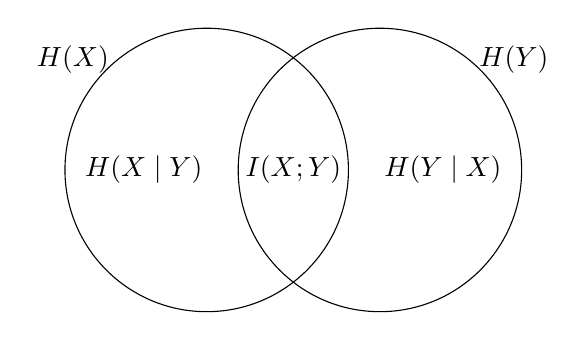
\begin{tikzpicture}[scale=1.0]
\def\r{1.8}
\draw (0,0) circle (\r);
\draw (2.2,0) circle (\r);
\node at (-1.7,1.4) {$H(X)$};
\node at (3.9,1.4) {$H(Y)$};
\node at (1.1,0) {$I(X;Y)$};
\node at (-0.8,0) {$H(X\mid Y)$};
\node at (3.0,0) {$H(Y\mid X)$};
\end{tikzpicture}
\caption{$H(X)$ and $H(Y)$ with overlap $I(X;Y)$.}
\end{figure}

%
% Section: Huffman Algorithm
%

\section{Huffman Algorithm}
\label{sec:Huffman-Algorithm}

From a practical point of view, there exists an algorithm, called \emph{Huffman algorithm}, that provides a method to build compact prefix-free codes given a probability distribution. For simplicity, we will study first the particular case of constructing binary prefix-free codes, and later I will provide its generalization to the case of D-ary prefix-free codes.

\begin{algorithm}
\caption{Huffman Algorithm}
\label{alg:Huffman}
\begin{algorithmic}
\Procedure{Huffman}{$Q$}
    \State $T \gets$ empty tree
    \For {$i \gets 1, d(Q) - 1$}
        \State allocate a new node $z$
        \State z.left = x = EXTRACT-MIN(Q)
        \State z.rigth = y = EXTRACT-MIN(Q)
        \State z.freq = x.freq + y.freq
        \State INSERT(Q, z)
    \EndFor
    \State \textbf{return} $T$
\EndProcedure
\end{algorithmic}
\end{algorithm}

The algorithm (see Algorithm \ref{alg:Huffman}) expects as input a source alphabet $\mathcal{S}=\left\{ s_{1},s_{2},\ldots,s_{q}\right\}$ and their corresponding probabilities $P = \left\{ p_{1}, p_{2}, \ldots, p_{q} \right\}$. For simplicity, $Q = \left\{ (s_{1}, p_{1}), (s_{2}, p_{2}), \ldots, (s_{q}, p_{q}) \right\}$ will merge both sets into a single one. The algorithm works by constructing a binary tree $T$, similar to the one used in the proof of Theorem \ref{th:Kraft-Inequality}. The algorithm requires $d(Q) - 1$ iterations to finish. During each iteration, the two elements with the lowest probability are selected and removed from set $Q$, and a new tree node $z$ is created, with the addition of the removed values, and added to the set $Q$. Once the tree has been constructed, we have to perform a tree transversal assigning a $0$ to each left branch, and a $1$ to each right branch, until we reach a leaf.

\begin{example}
Assume we have the source alphabet $\mathcal{S}=\left\{a, b, c, d, e, f\right\}$ with the associated probabilities $P = \left\{0.35, 0.16, 0.08, 0.12, 0.06, 0.23 \right\}$. In Figure \label{fig:Huffman-Algorithm} are depicted the contents of the set $Q$ and the tree $T$ for each iteration of the algorithm. At the end of the algorithm, if we perform a traversal of the $T$ tree, we will get the following prefix-free compact code for the source alphabet $S$: 

\bigskip

\centering
\begin{tabular}{l l}
\toprule
\textbf{Source Word} & \textbf{Code Word} \\
\midrule
a & 11   \\
b & 00   \\
c & 1011 \\
d & 100  \\
e & 1010 \\
f & 01   \\
\bottomrule
\end{tabular}

\bigskip

% The expected length of the code is $L = 2.4$ , and its entropy is $\mathcal{H} \approx 2.34$. Since the set of probabilities is not D-adic ...

% % Q: Shall I mention the expected length of a uniform code?

\end{example}

% \begin{figure}[h]
% \centering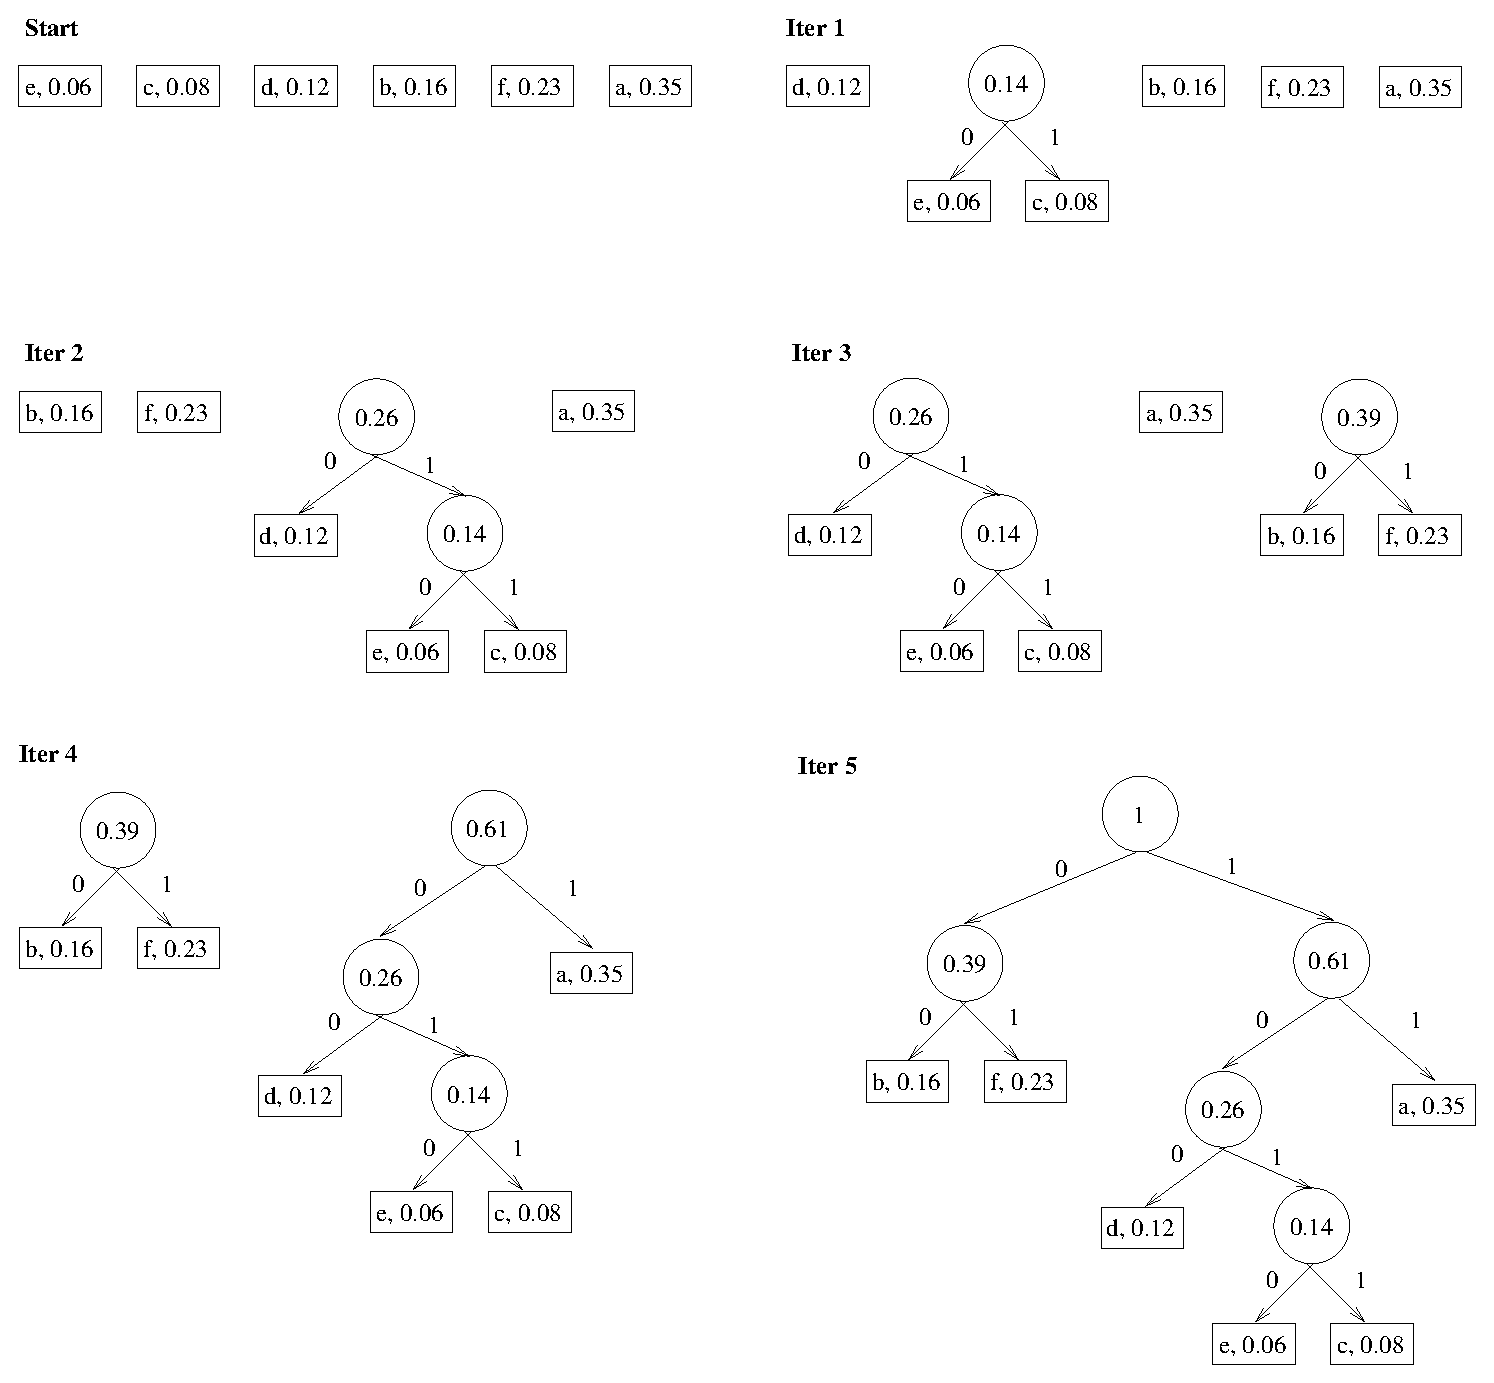
\includegraphics[scale=0.5]{huffman}
% \caption{\label{fig:Huffman-Algorithm}Huffman Algorithm}
% \end{figure}

% \emph{This order is arbitrary; switching the left and rigth child of any node yields a different code of the same cost}

% % Lemma would be better

% \begin{proposition}
% Given the probability is ...
% \end{proposition}
% \begin{proof}
% {\color{red} TODO}
% \end{proof}

% The next theorem shows the optimality of the Huffman coding.

% \begin{theorem}
% If $C$ is a Huffman code then $C$ is compact.
% \end{theorem}
% \begin{proof}
% {\color{red} TODO}
% \end{proof}

% {\color{red} TODO: Rewrite the following paragraphs}

% \emph{So not only is this code optimal in the sense that no other feasible code performs better, but it is very close to the theoretical limit established by the entropy}

% \emph{Although we have proved the theorem for a binary alphabet, the proof can be extended to establishing optimality of the Huffam coding algorithm for a D-ary alphabet as well.}

% {\color{red} TODO: show how to extend the algorithm to D-ary codes}

% \emph{Then -ary Huffman algorithm uses the {0, 1, ..., n-1} alphabet to encode message and build an n-ary tree [...] the same algorithm applies as for binary codes, except that the n least probable symbols are taken together , instead of just the 2 least probable. Note that for n greater than 2, not all sets of source words  can properly form an n-ary tree for Huffman coding. In this case, additional 0-probability place holders must be added. This is because the tree must form and n to 1 contractor; for binary coding, this is a 2 to 1 contractor, and any sized set can form such a contractor. If the number fo source words is congruent to 1 module n-1, then the set of source words will form a proper Huffman tree.}

% {\color{red} Mention arithmetic coding}

%
% Discretization of Continuous Variables
%

\section{Discretization of Continuous Variables}
\label{sec:discretization_continuous_variables}

When summarizing large masses of raw data, it is often useful to distribute the data into classes, or categories, and to determine the number of individuals belonging to each class, called absolute frequency. The following definition formally introduces this concept.

\begin{definition}
Let $\mathcal{S}$ be a population consisting of $n$ individuals, and let a variable $X: \mathcal{S} \rightarrow \mathcal{D}$ represent the mapping of individuals in $\mathcal{S}$ to values in the set $\mathcal{D}$, where $k$ is the cardinality of $\mathcal{D}$. The \emph{absolute frequency}\index{Absolute frequency}, also known simply as \emph{frequency}, denoted by $n_i$ for $1 \leq i \leq k$, quantifies the number of individuals in $\mathcal{S}$ for which $X$ assigns the value corresponding to the $i$-th category of $\mathcal{D}$.
\end{definition}

The sum of the frequencies must be equal to population size, that is, $\sum_{i=1}^k n_i = n$.

If the variable $X$ is continuous, the elements of $\mathcal{D}$ are referred to as \emph{class intervals}\index{Class interval}. The endpoints of these intervals are known as \emph{class limits}\index{Class limits}; the smaller number is termed the \emph{lower class limit}\index{Lower class limit}, and the larger number, the \emph{upper class limit}\index{Upper class limit}. A \emph{class interval}\index{Class interval} that lacks either an upper or a lower class limit is known as an \emph{open class interval}\index{Open class interval}. The \emph{width}\index{Class interval width} of a class interval is defined as the difference between the upper and lower class boundaries, denoted by $a_i = e_i - e_{i-1}$. The \emph{class mark}\index{Class mark}, or the midpoint of a class interval, is calculated as $a_i = \frac{e_i + e_{i-1}}{2}$. It is assumed that all observations within a specific class interval are equivalent concerning their categorical assignment. Refer to Section \ref{sec:discretization_algorithms} for more information about how to discretize a continous variable into discrete intervals.

\begin{example}
In a study measuring adult heights within a community, researchers record heights ranging from 150 cm to 200 cm and organize them into 10 cm class intervals: 150-159 cm, 160-169 cm, 170-179 cm, 180-189 cm, and 190-199 cm. Each interval's lower and upper class limits are respectively the start and end points, such as 150 cm and 159 cm for the first interval. If the last interval had no specified upper limit, it would be considered an open class interval. The class width, typically 10 cm, is the operational span between boundaries, and the class mark, calculated as the midpoint of each interval (e.g., 154.5 cm for the first interval), provides a central value for summarizing data within that range.
\end{example}

A tabular arrangement of data by classes together with the corresponding class frequencies is called a frequency distribution, or frequency table.

\begin{definition}
Let $\mathcal{S}$ be a population consisting of $n$ individuals, and let $X: \mathcal{S} \rightarrow \mathcal{D}$ be a variable that maps individuals in $\mathcal{S}$ to $k$ distinct values of the set $\mathcal{D}$. A \emph{frequency distribution}\index{Frequency distribution} is represented the set of pairs $\{(d_i, n_i) : 1 \leq i \leq k\}$, where $d_i$ denotes the $i$-th interval and $n_i$ represents the number of individuals from $\mathcal{S}$ whose value under $X$ falls within the interval $d_i$.
\end{definition}

Frequency distributions are useful for statistical analysis and helps in visualizing data by grouping values, which simplifies the understanding of distribution and central tendencies within the data.

The relative frequency of a class is the frequency of the class divided by the total frequency of all classes

\begin{definition}
Let $\mathcal{S}$ be a population consisting of $n$ individuals, and let a variable $X: \mathcal{S} \rightarrow \mathcal{D}$ represent the mapping of individuals in $\mathcal{S}$ to values in the set $\mathcal{D}$, where $k$ is the cardinality of $\mathcal{D}$. The \emph{relative frequency}\index{Relative frequency}, denoted by $f_i$, is the ratio $f_i = \frac{n_i}{n}$ for $1 \leq i \leq k$.
\end{definition}

The sum of the relative frequencies is equal to one, that is, $\sum_{i=1}^k f_i = 1$.

The total frequency of all values less than the upper class boundary of a given class interval is called the cumulative frequency up to and including that class interval.

\begin{definition}
Let $\mathcal{S}$ be a population consisting of $n$ individuals, and let a variable $X: \mathcal{S} \rightarrow \mathcal{D}$ represent the mapping of individuals in $\mathcal{S}$ to values in the set $\mathcal{D}$, where $k$ is the cardinality of $\mathcal{D}$. The \emph{cumulative frequency}\index{Cumulative frequency}, denoted by $N_i$ for $1 \leq i \leq k$, represents the total number of individuals in $\mathcal{S}$ for which $X$ assigns a value less than or equal to the upper limit of the $i$-th category of $\mathcal{D}$. This is mathematically expressed as $N_i = \sum_{j=1}^i n_j$, where $n_j$ is the absolute frequency of the $j$-th category.
\end{definition}

By accumulating the frequencies up to each category or interval, cumulative frequencies provides a running total that shows how many data points fall below a certain value.

\subsubsection*{Discretization Algorithms}

Let $\mathcal{X}$ a continuous random variable that follows a probability density function $P_\mathcal{X}$, and assume we have collected $n$ independent and identically distributed samples $\bold{x} = \{x_1, \ldots, x_n\}$ from $\mathcal{X}$. We are interested in computing the length of a compressed version of $\bold{x}$ using an optimal compressor. Unfortunately, and except for some degenerate distributions, there is no lossless compression algorithm that produces a string with fewer bits than encoding directly the elements $\bold{x}$. Compression algorithms for continuous data only work in case that the elements of $\bold{x}$ are not independent, as it is the case with images or sound. But, if this is not the case, the only option available to compress $\bold{x}$ is to use a lossy compression algorithm, where some information is lost.

We are looking for an algorithm to produce a finite non-overlapping partition of $m$ discrete intervals $D=\{ [d_o, d_1], (d_1, d_2], \ldots, (d_{m-1}, d_m] \}$, where $d_o = \min{\bold{x}_j}$, and $d_m = \max{\bold{x}_j}$, and $d_i < d_{i+1}$ for $i = 0, 1, \ldots, m-1$, assign a unique label to each interval, and encode the elements of $\bold{x}$ using this labeling schema. As compression algorithm we will use an optimal length code given the relative frequencies of the labels in the encoded vector. In this sense, our goal is to have a collection of intervals with sufficiently number of samples (so they are statistically significant) and that the distribution of frequencies resembles the original probability distribution $P_\mathcal{X}$.

A discretization algorithm is a mapping between a (possibly huge) number of numeric values and a reduced set of discrete values, and so, it is a process in which some information is potentially lost. The choice of discretization algorithm is something that could have a high impact in the practical computation of the nescience. We are interested in a discretization algorithm that produces a large number of intervals (low bias), with a large number of number of observations per interval (low variance). Common techniques include \emph{equal width discretization}, \emph{equal frequency discretization} and \emph{fixed frequency discretization}. However, these techniques require the optimization of an hyperparameter, and so, they are not suitable for our purposes.

In a \emph{proportional discretization approach} the number of intervals $m$ and the number of observations per interval $s$ are equally proportional to the number of observations $n$. The algorithm starts by sorting the values of $\bold{x}_j$ in ascending order and then discretizing them into $m$ intervals of approximately $s$ (possibly identical) values each. In this way, as the number of training observations increases, both interval frequency and number of intervals increases, taking advantage of the larger number of observations. In the same way, when the number of observations decreases, we reduce both.

%
% References
%

\section*{References}

Core references for the chapter "Coding"

\cite{cover2012elements}: Cover and Thomas is the standard reference for modern information theory. It introduces entropy, mutual information, source and channel coding theorems, and provides the theoretical basis for coding.

\cite{abramson1963information}: Abramson's book is a classic early text that presents coding theory in an accessible way. It is useful for historical perspective and for understanding the development of the main coding ideas.

\cite{kraft1949device}: Kraft’s thesis introduces the Kraft inequality, a cornerstone result for the theory of uniquely decodable prefix codes.

\cite{mcmillan1956two}: McMillan extends Kraft's result to a more general form, establishing the Kraft-McMillan inequality fundamental to coding theory.

\cite{gersho2012vector}: Gersho and Gray provide the standard reference on quantization methods used in lossy compression, important for bridging coding theory with practical applications.

\cite{lloyd1982least}: Lloyd’s algorithm (often rediscovered as k-means) is a central method for quantization and lossy compression. It provides a concrete link between coding and clustering.

\cite{li2013introduction}: Li and Vitányi’s book is the definitive source on Kolmogorov complexity, linking coding theory with randomness and algorithmic information. It is essential for connecting coding to the broader framework of nescience.

% \begin{verbatim}

% % Rice's rule

% A common rule of thumb for determining the number of bins in a histogram is Rice’s rule, which suggests using approximately 2n^1/3 bins, where n is the sample size. This heuristic strikes a balance between over-smoothing and over-fitting and has been widely adopted in introductory statistics texts as a practical default choice for discretization \cite{freedman1978statistics}.

% Freedman, D., Pisani, R., & Purves, R. (1978). Statistics (2nd ed.). New York, NY: W. W. Norton. (Section 6.3: binning rules including “twice the cube root of n”).

% @book{freedman1978statistics,
%   title={Statistics},
%   author={Freedman, David and Pisani, Robert and Purves, Roger},
%   year={1978},
%   publisher={W. W. Norton \& Company}
% }

% % Jeffreys smoothing

% @article{krichevsky1981performance,
%   title={The performance of universal encoding},
%   author={Krichevsky, R. E. and Trofimov, V. K.},
%   journal={IEEE Transactions on Information Theory},
%   volume={27},
%   number={2},
%   pages={199--207},
%   year={1981},
%   publisher={IEEE}
% }

% To avoid degenerate estimates when computing code lengths from finite samples, we apply a Bayesian smoothing procedure known as the **Krichevsky-Trofimov (KT) estimator**, also called **Jeffreys prior smoothing**. This method assigns a prior weight of $1/2$ to each possible outcome, resulting in probability estimates of the form $(n_i+1/2)/(N + k/2)$, where $n_i$ is the count of symbol $i$, $N$ the sample size, and $k$ the alphabet size. This estimator was introduced in the information theory literature by Krichevsky and Trofimov\~\cite{krichevsky1981performance}, and it is known to yield nearly optimal universal coding performance.

% % Trimmed core range

% @book{huber1981robust,
%   title={Robust Statistics},
%   author={Huber, Peter J.},
%   year={1981},
%   publisher={John Wiley \& Sons}
% }
% When discretizing continuous variables, extreme outliers can distort the binning process, leading to empty or uninformative intervals. To address this, we use a **trimmed core range**, where a small fraction (e.g., 0.5\%) of the data at each tail is excluded when defining the binning range. This approach comes from the broader field of **robust statistics**, which develops methods that are less sensitive to outliers. The idea of trimming as a robustness technique was systematically developed in Huber's classic monograph\~\cite{huber1981robust}.

% \end{verbatim}




